\documentclass[./00PhotoBox.tex]{subfiles}
\graphicspath{{\subfix{./img/}}}
\begin{document}

\chapter{Software-Entwicklung}
Für die Steuerung der Kameras und die anschließende Berechnung des 3D-Modelles muss ein Steuerungssoftware für das Kamerasystem und eine entsprechende Schnittstelle zu einer \gls{SfM}-Software geschaffen werden. Diese Entwicklung erfolgte hauptsächlich in Python in Form von Prototyping. Das Kapitel beschreibt die Anforderungen an die Software in \autoref{sec:Anforderungsanalyse} und die zu implementierenden Anwendungsfälle (\autoref{sec:Anwendungsfallmodellierung}). Abschließend wird die Implementation (\autoref{sec:Implementierung}) erarbeitet.
\todo{erst Anwendungsfälle, dann Anforderungen?}

\section{Anforderungsanalyse}
\label{sec:Anforderungsanalyse}

\subsection{Funktionale Anforderungen}
\begin{enumerate}[label=F\arabic*]
    \item Die Kameras sollen zeitgleich auslösbar sein. Es soll möglichst ver\-zögerungs\-frei ausgelöst werden.
    \item Die Steuerung soll auch unabhängig von anderen Geräten möglich sein, beispielsweise per Tastensteuerung.
    \item Der Status des Systemes soll für den Nutzer erkennbar sein - auch ohne Anschluss eines Computers.
    \item Es sollen Passpunkte automatisch gefunden und für die Bestimmung der äußeren Orientierung genutzt werden.
    \item Die Bilder sollen scharf und fokussiert sein. Die Belichtung soll automatisch erfolgen, jedoch die Helligkeit der Bilder identisch sein.
\end{enumerate}

\subsection{Schnittstellen}
\begin{enumerate}[label=S\arabic*]
    \item Die Daten sollen intern gespeichert werden.
    \item Eine Speicherung auf tragbaren Speichermedien wie USB-Sticks soll möglich sein.
    \item Eine direkte Übertragung an \gls{SfM}-Software soll möglich sein.
\end{enumerate}

\subsection{Nicht-funktionale Anforderungen}
\begin{enumerate}[label=N\arabic*]
    \item Die Erfassung soll ohne weitere Hardware möglich sein. Das System soll unabhängig von Netzwerkanschlüssen etc. sein.
    \item Alle Kommunikation soll über WLAN erfolgen.
\end{enumerate}

\section{Anwendungsfallmodellierung}
\label{sec:Anwendungsfallmodellierung}

Entsprechend der benötigten Schritte aus \autoref{c:photogrammetrie} und \autoref{img:ablauf} wurde die Anwendungsfälle, die die Benutzeroberfläche ermöglichen soll, im Anwendungsfall-Dia\-gramm in \autoref{img:anwendungsfall} zusammengetragen. Entsprechend der Anforderung, dass das System einfach in der Bedienung gehalten sein soll, ist die Anzahl der verschiedenen Anwendungsälle gering.

\begin{figure}
    \centering
    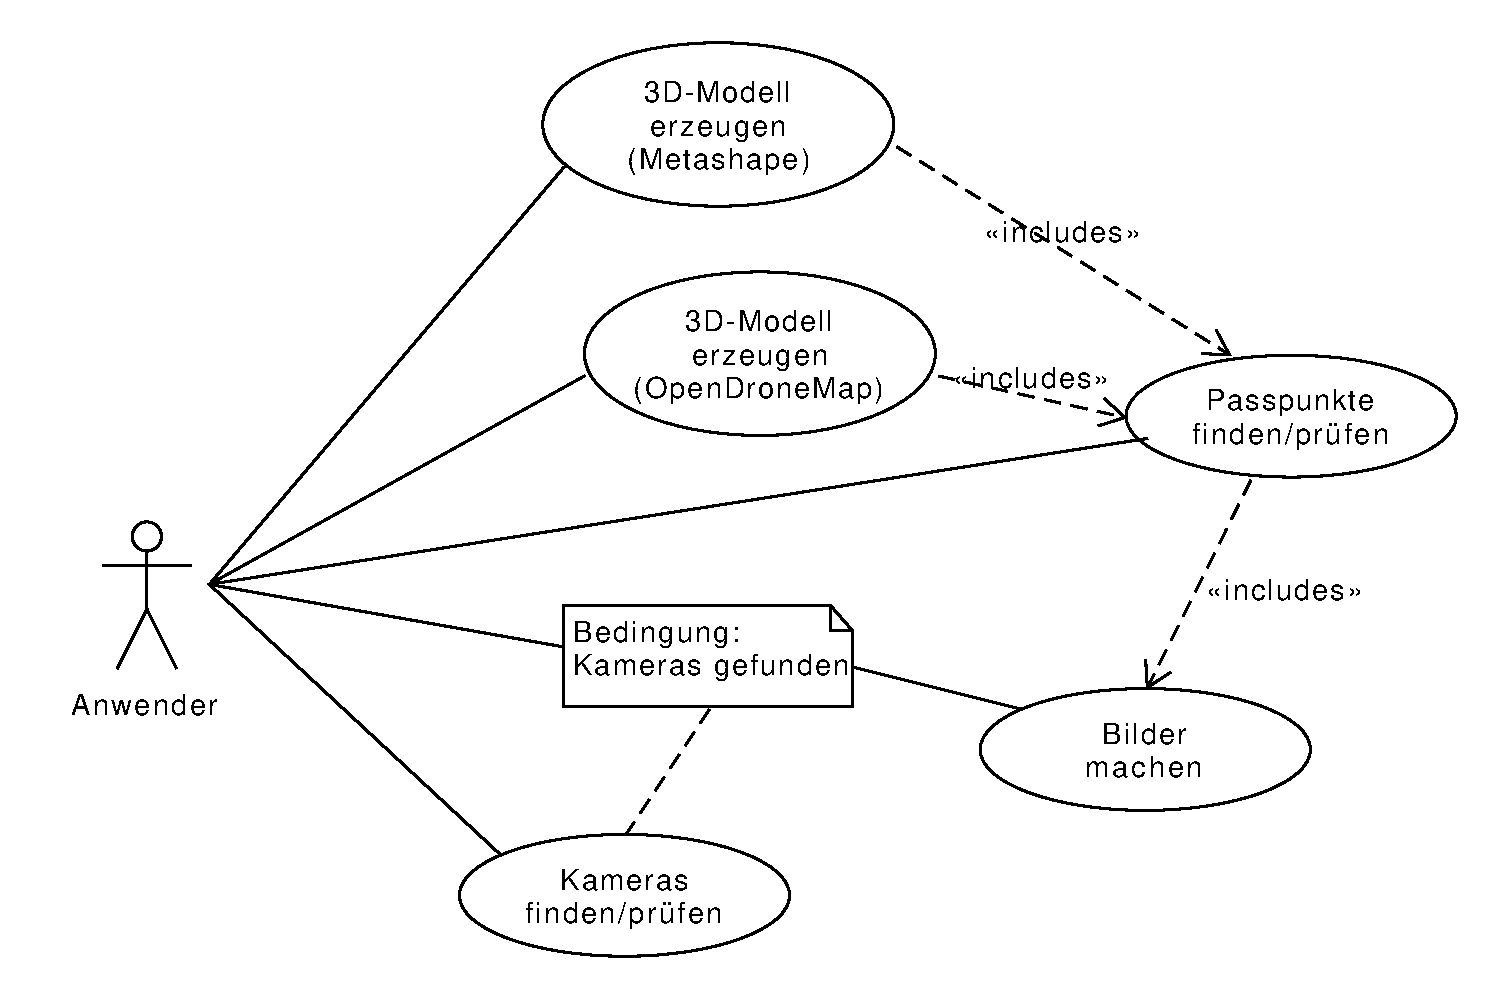
\includegraphics[width=1\textwidth]{./img/uml/uml_usecases.pdf}
    \caption{Anwendungsfall-Diagramm} %Bildunterschrift
    \label{img:anwendungsfall} %ID fürs Bild
\end{figure}

Aus den benötigten Daten wurde das Domänen-Klassendiagramm aus \autoref{img:dokladia} erzeugt. Dieses zeigt vor allem die Abhängigkeiten der einzelnen Datensätze untereinander.

\begin{figure}
    \centering
    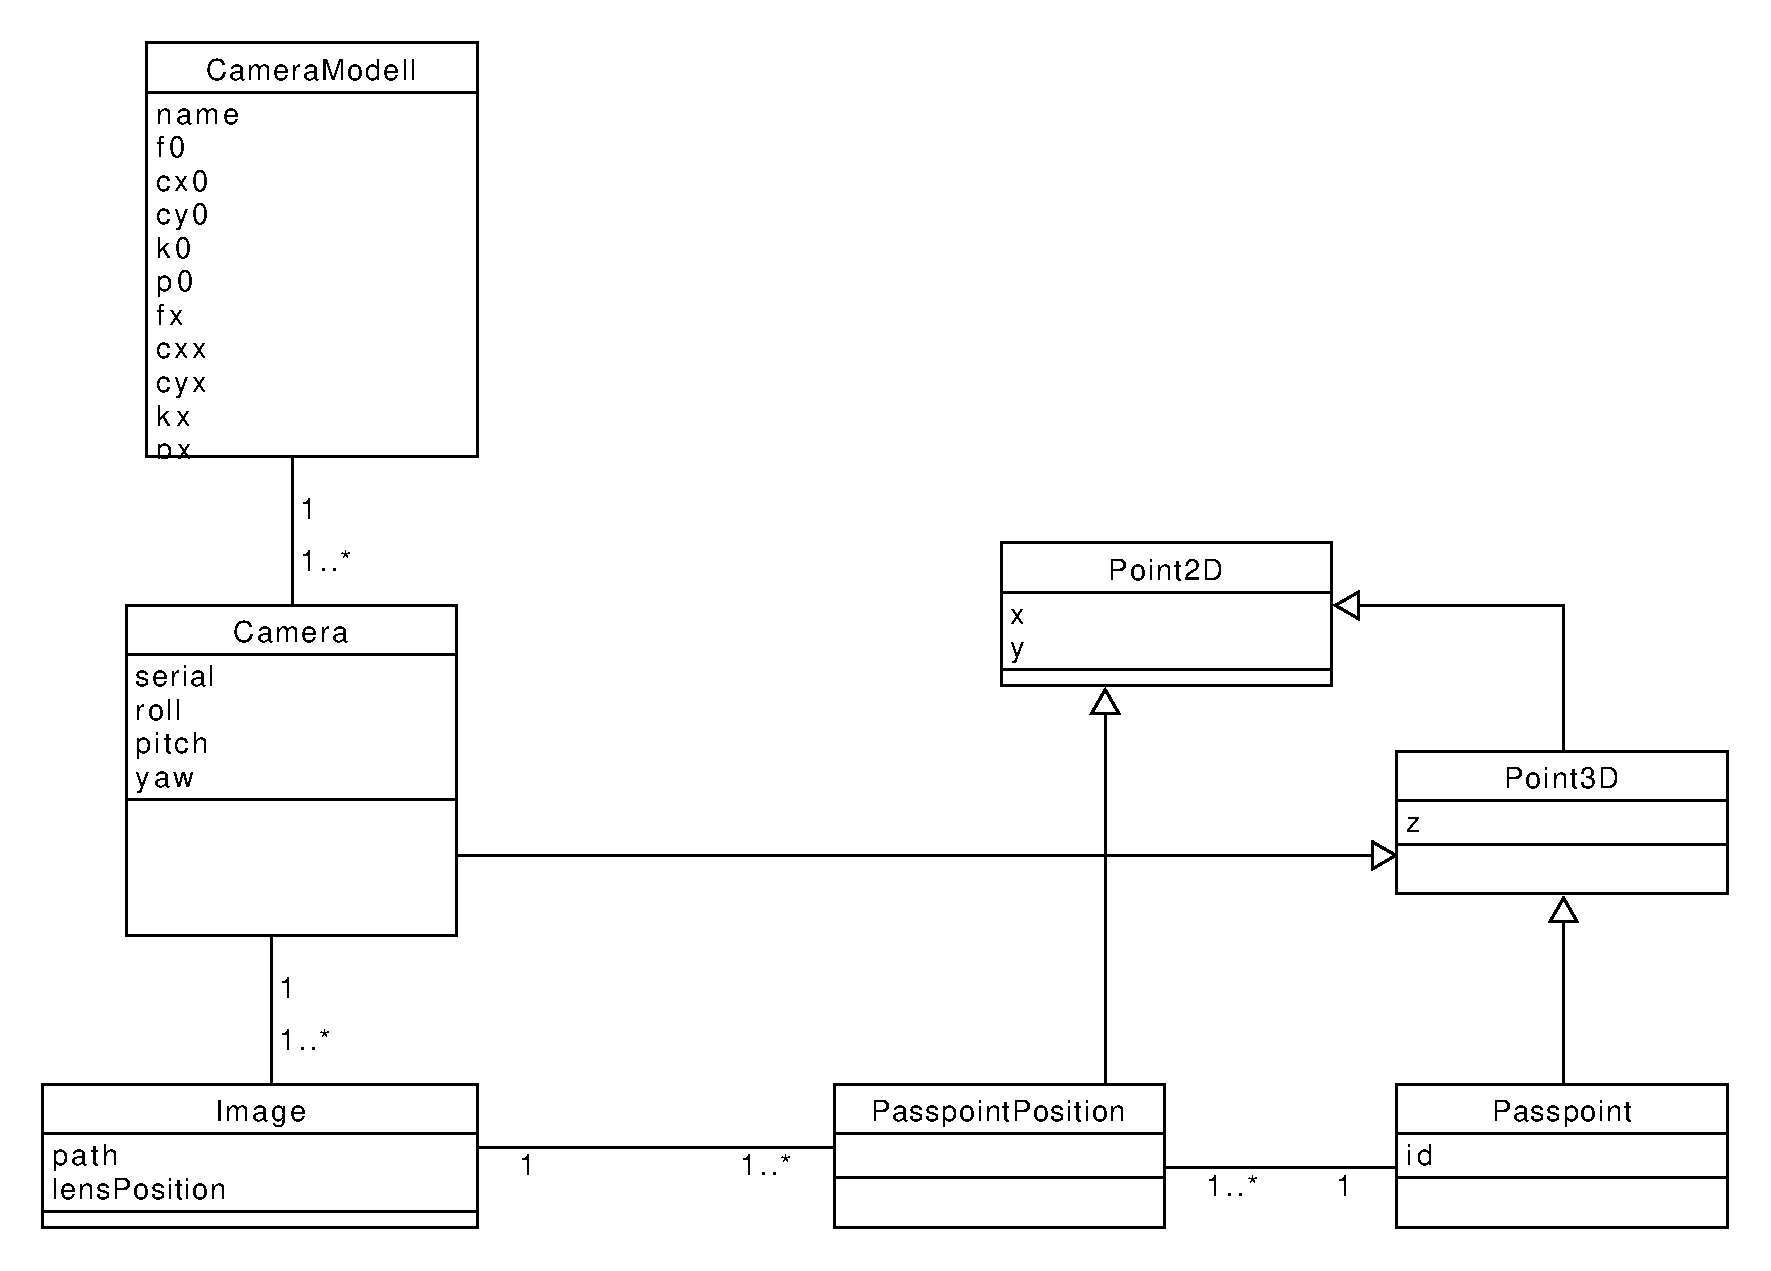
\includegraphics[width=1\textwidth]{./img/uml/uml_domain.pdf}
    \caption{Domänen-Klassendiagramm} %Bildunterschrift
    \label{img:dokladia} %ID fürs Bild
\end{figure}

\section{Implementierung}
\label{sec:Implementierung}


Die Programmierung des Systemes erfolgte iterativ. Einzelne Arbeitspakete wurden in einem Jupyter-Notebook ausprobiert und dann, wenn dieser Schritt erfolgreich war, in den Gesamtworkflow integriert - teilweise sind diese im \autoref{c:voruntersuchungen} beschrieben. Größtenteils wurden der Python-Code objektorientiert und typisiert geschrieben. Die Teile, die auf einem Desktoprechner laufen sollen, wurden in Java geschrieben, da hier später die Einrichtung auf verschiedenen Rechnern und Plattformen einfacher ist.

Die Kommunikation innerhalb des Systemes ist in dem Ablaufdiagramm aus \autoref{img:uml_sequence_capture} dargestellt. Auf die Details der einzelnen Module wird in den folgenden Abschnitten eingegangen.


\begin{figure}
    \centering
    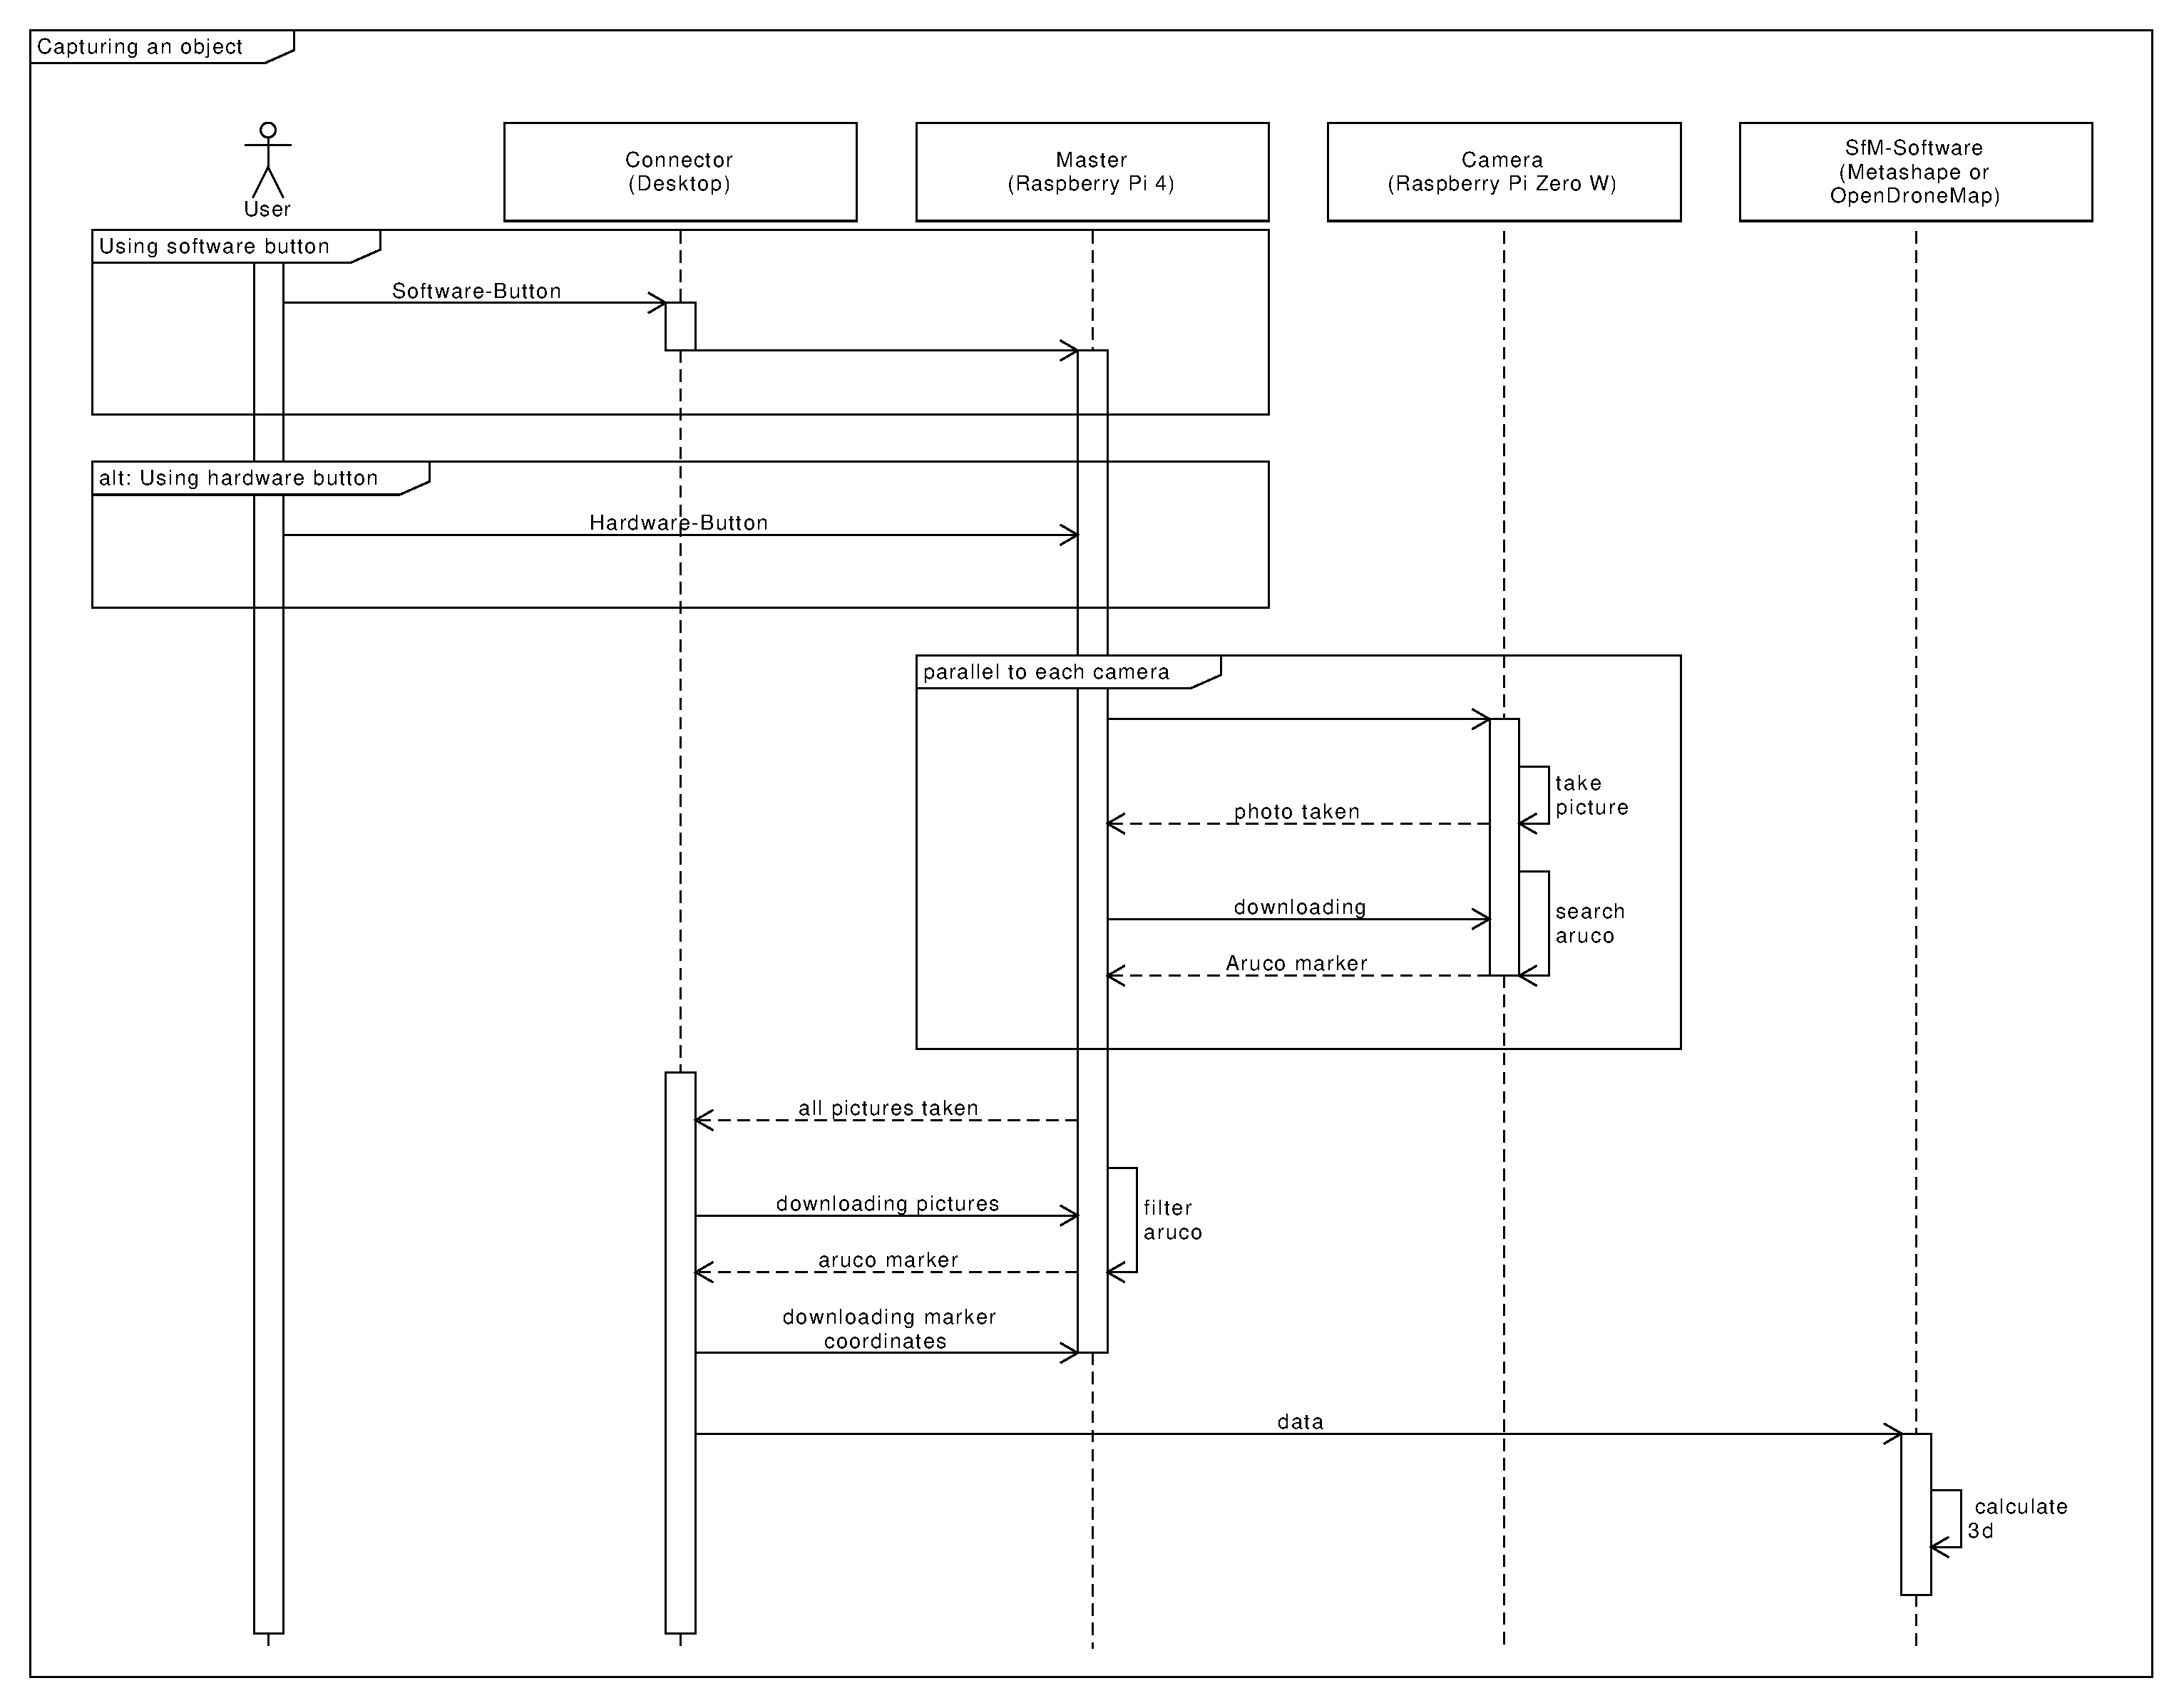
\includegraphics[width=1\textwidth]{./img/uml/uml_sequence_capture.pdf}
    \caption{Ablaufdiagramm zur Kommunikation bei der Aufnahme eines 3D-Modelles} %Bildunterschrift
    \label{img:uml_sequence_capture} %ID fürs Bild
\end{figure}


\subsection{Module auf den Raspberry Pi (Python)}
\todo{Plural von Raspberry Pi verdeutlichen}
Die Software auf den Raspberry Pi wurde in Python geschrieben. Hierbei wurde darauf geachtet, dass die Module möglichst unabhängig voneinander sind und nur über definierte Schnittstellen kommunizieren.

\subsubsection{Bibliotheken}
Es wurde, wenn möglich, auf fertige Python-Bibliotheken zurückgegriffen. Hierdurch sollte der Programmieraufwand verringert und auf bereits getesteten Code gesetzt werden. Außerdem greifen viele der Bibliotheken wie OpenCV oder NumPy auf hardwarenahere Berechnungen zurück, so dass der Geschwindigkeitsnachteil von Python nicht weiter ins Gewicht fällt. Die wichtigsten Bibliotheken sind:

\paragraph{OpenCV}
ist eine Bibliothek für Bildbearbeitung und maschinelles Sehen. Sie ist weit verbreitet und bietet viele photogrammetrische Funktionen. Hiermit wurde beispielsweise die Detektion von Markern durchgeführt und die Näherungswerte der Kameras berechnet.

\paragraph{NumPy}
bietet neben vielen weiteren Funktionen die Möglichkeit der Matrizenrechnung. Diese wurde für viele Berechnungen benötigt, beispielsweise für die Berechnungen der Kamera-Projektionen.

\paragraph{SciPy}
wurde für die Berechnung der Bündelblockausgleichung verwendet. Der manuelle Ansatz mit den Formeln aus \cite{luhmann} unter Nutzung von NumPy war sehr ressourcenlastig. Unter Verwendung von SciPy und der Projektionsgleichung konnte die Berechnungsdauer stark dezimiert werden.

\paragraph{Flask}
wurde genutzt um die Weboberfläche und die Datendownloads bereitzustellen. Hiermit wurde ein Webserver aufgesetzt, der die Daten der Kameras anzeigt und die Steuerung ermöglicht.

\subsubsection{Allgemeine Module}
Es wurden einige Klassen erstellt, die in allen Modulen genutzt wurden. Diese sind in \autoref{img:uml_common} dargestellt. Diese steuern allgemeine Funktionen wie das Logging und das Auslesen der Konfiguration. Außerdem legen die Interfaces die Struktur der Datenübertragung zwischen den Raspberry Pi fest. \todo{Plural Raspberry Pi verdeutlichen}

\begin{figure}
    \centering
    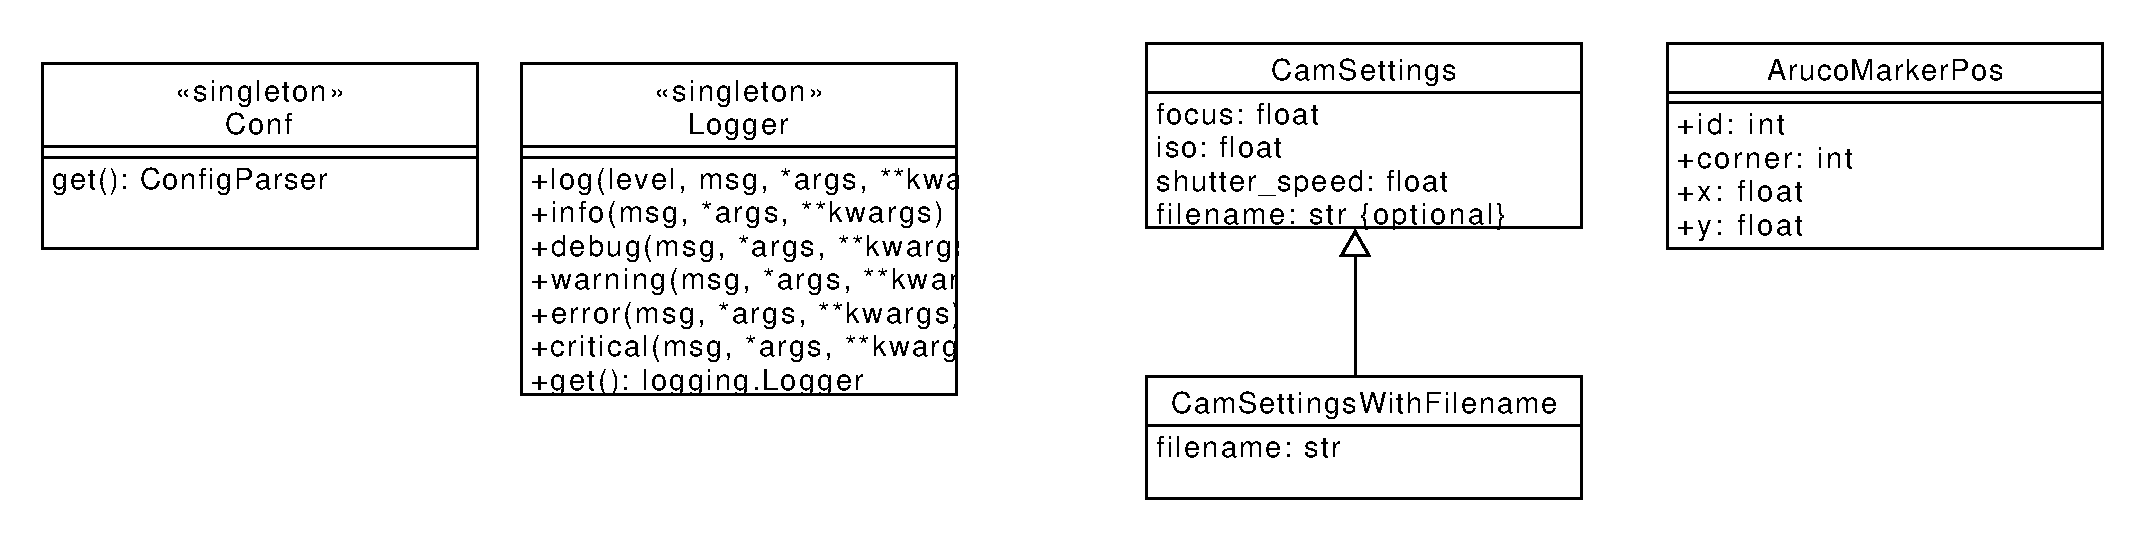
\includegraphics[width=1\textwidth]{./img/uml/uml_common_classdiagramm.pdf}
    \caption{Common} %Bildunterschrift
    \label{img:uml_common} %ID fürs Bild
\end{figure}
\todo{UML vervollständigen}


\subsubsection{Master-Steuerung}

Auf einem Raspberry Pi 4 läuft die Gesamtsteuerung des Systemes. Dieses stellt Schnittstellen zur Steuerung auf drei verschiedenen Wegen bereit: per Taster, per Weboberfläche und per Socket-Verbindung. Außerdem stellt es die Daten per REST-Schnittstelle zur Verfügung. Die Klassen sind in \autoref{img:master} dargestellt.

Die Steuerung per Taster ermöglicht einfache Aufgaben wie das Suchen von Kameras, das Aufnehmen von Bilder und die Aktivierung des Standbys bzw. das Herunterfahren des Systems auch ohne PC durchzuführen. Die Weboberfläche ermöglicht die komplette Steuerung, das Konfigurieren sowie das Anzeigen und Herunterladen der Bilder. Die Socket-Verbindung ermöglicht die Kommunikation mit der Desktop-Software und die Steuerung hierüber.

Der Raspberry Pi sammelt die Daten der einzelnen Kameras und stellt diese zur Weiterverarbeitung zur Verfügung. Die Datenübertragung an die Desktop-Software erfolgt über die REST-Schnittstelle. Alternativ kann auch ein USB-Stick an dem Raspberry Pi angesteckt werden oder die Daten über die Weboberfläche manuell heruntergeladen werden.

\begin{figure}
    \centering
    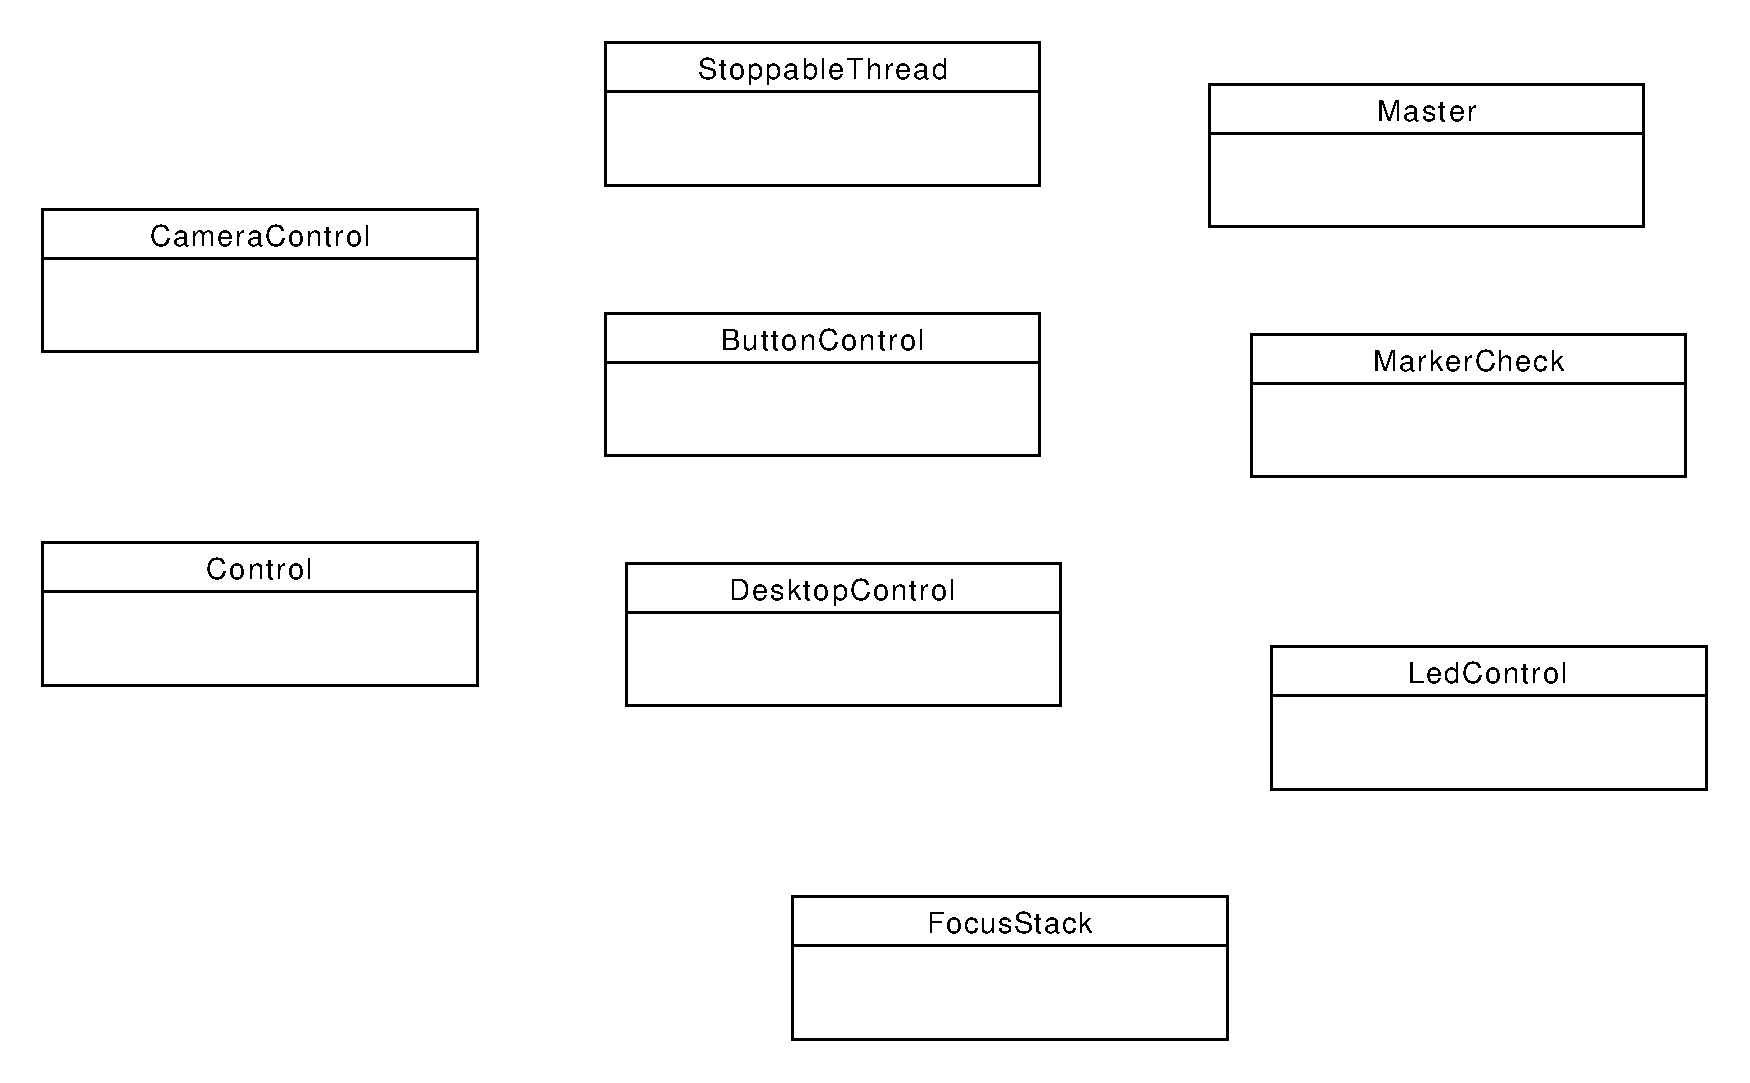
\includegraphics[width=1\textwidth]{./img/uml/uml_master_classdiagramm.pdf}
    \caption{Master} %Bildunterschrift
    \label{img:master} %ID fürs Bild
\end{figure}


\subsubsection{Kamera-Steuerung}
Die Raspberry Pi Zero W übernehmen die Steuerung der Kameras. Hierfür wurde ein Modul entwickelt das die Kameras steuert, die Bilder aufnimmt und anschließend dem steuernden Raspberry zur Verfügung stellt. Die Klassen sind in \autoref{img:uml_camera} dargestellt. Neben einer einfachen Benutzeroberfläche in Form einer über Flask bereitgestellten Website, erfolgt die Kommunikation bzw. Steuerung über eine REST-Schnittstelle zur Datenübertragung und eine Socket-Verbindung, die auf Broadcast-Nachrichten vom steuernden Raspberry Pi 4 wartet. Außerdem übernimmt der Raspberry Pi Zero W die Identifizierung von ArUco-Markern in den aufgenommenen Bildern.

\begin{figure}
    \centering
    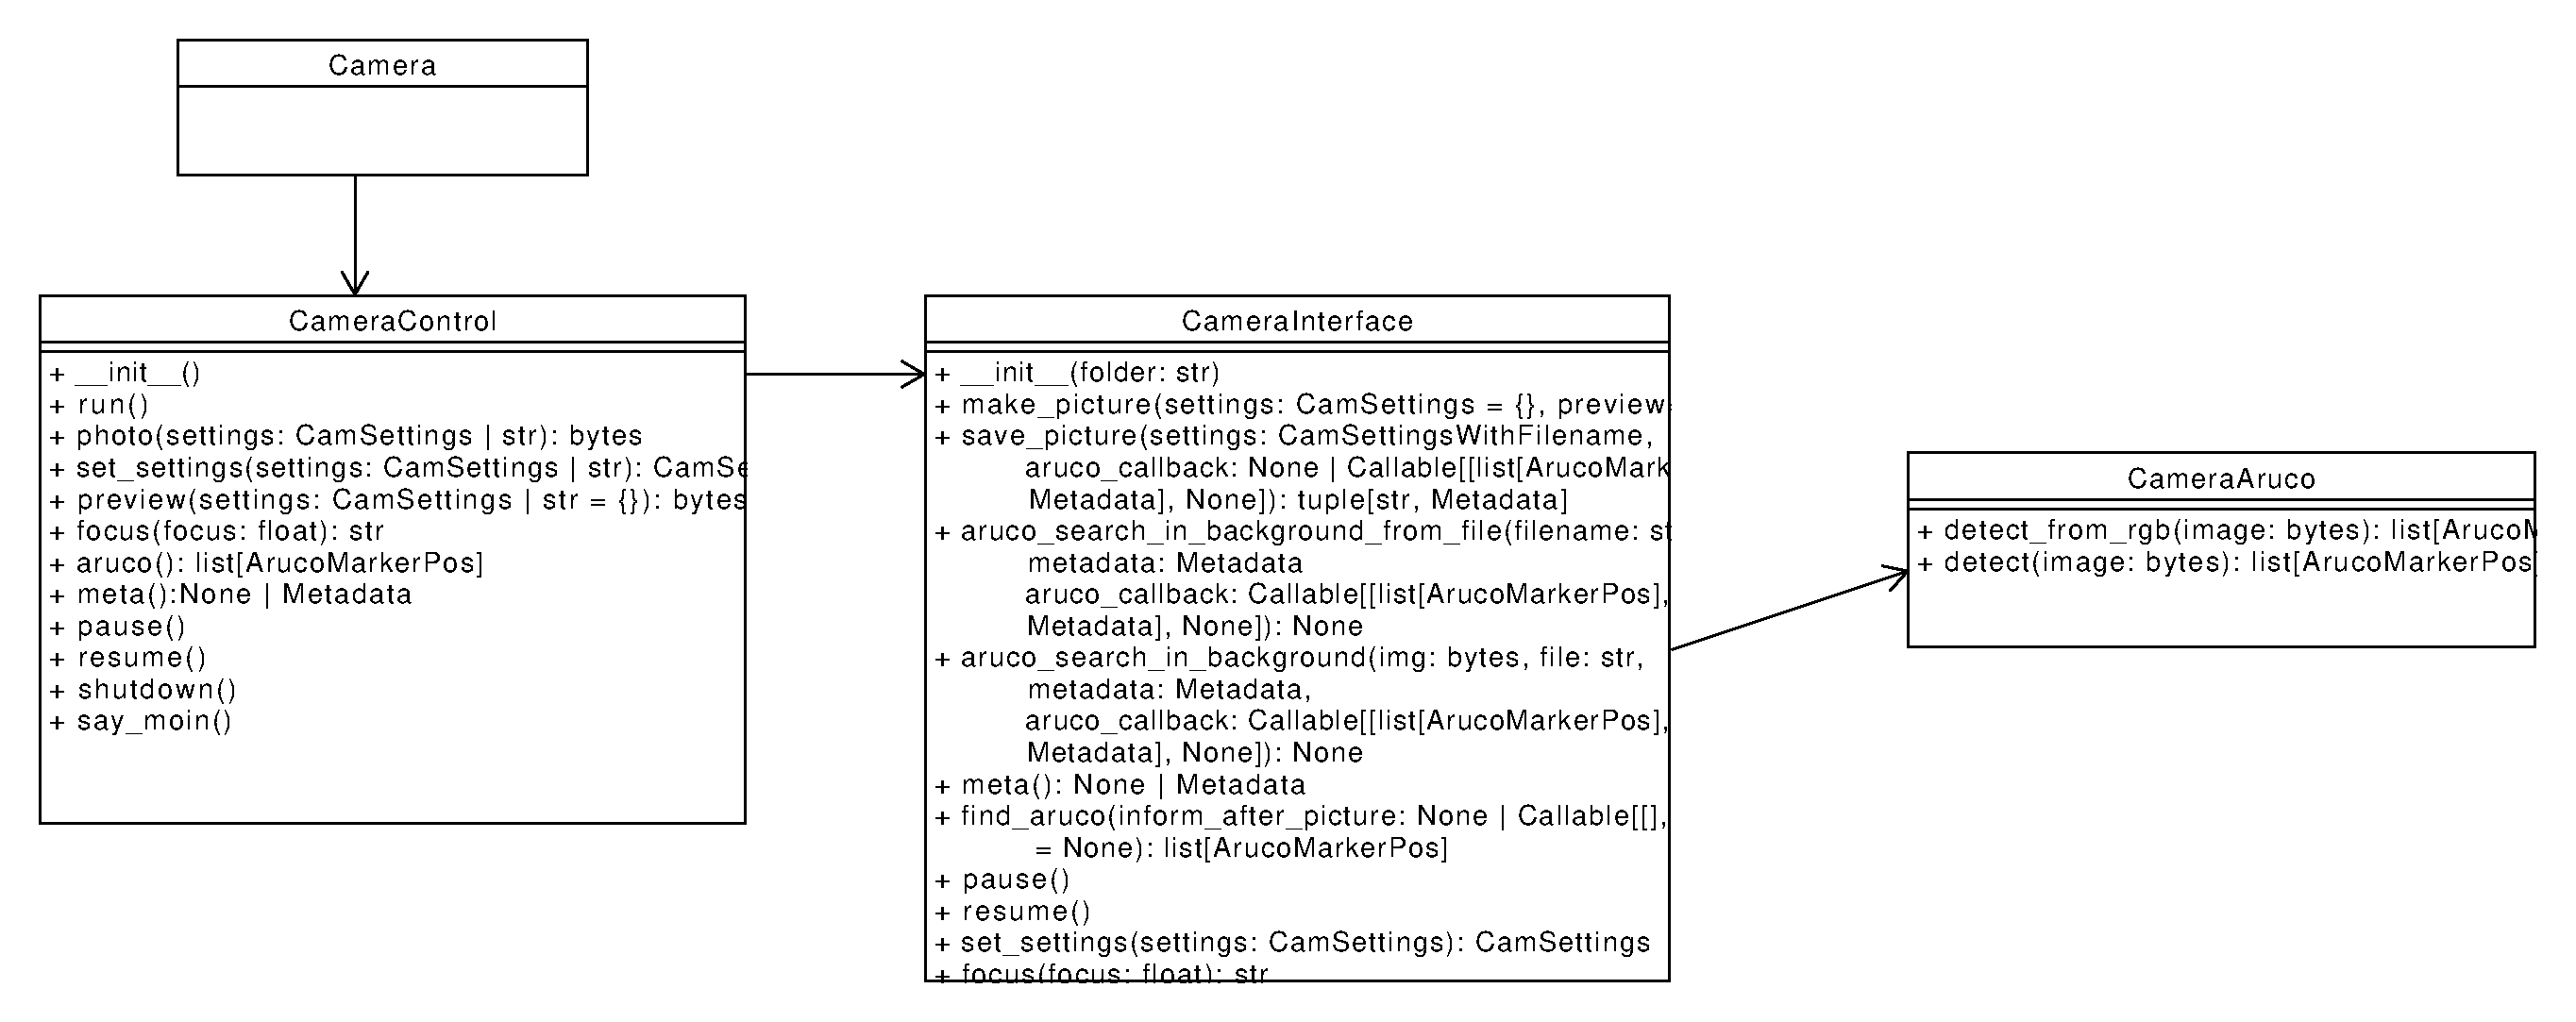
\includegraphics[width=1\textwidth]{./img/uml/uml_camera_classdiagramm.pdf}
    \caption{Camera} %Bildunterschrift
    \label{img:uml_camera} %ID fürs Bild
\end{figure}


\subsubsection{Desktop-Programm (Java)}
Die Desktop-Software dient zur Steuerung des Systems und zur automatischen Über\-tragung der Daten an die \gls{SfM}-Software. Die Klassen sind in \autoref{img:uml_connector} dargestellt. Sie wurden in Java geschrieben, um eine einfache Installation auf verschiedenen Betriebssystemen zu ermöglichen. Die Kommunikation erfolgt über eine Socket-Verbindung zum Raspberry Pi 4. Neben der Übertragung der Bilder an die \gls{SfM}-Software ermöglicht die Software das Starten von Aufnahmen. Ein Screenshot der Benutzeroberfläche ist in \autoref{img:screenshot_connector} dargestellt. Die Software unterstützt als \gls{SfM}-Software aktuell Agisoft Metashape und OpenDroneMap, jedoch ist die Schnittstelle so gestaltet, dass auch andere Software ergänzt werden könnte.


\begin{figure}
    \centering
    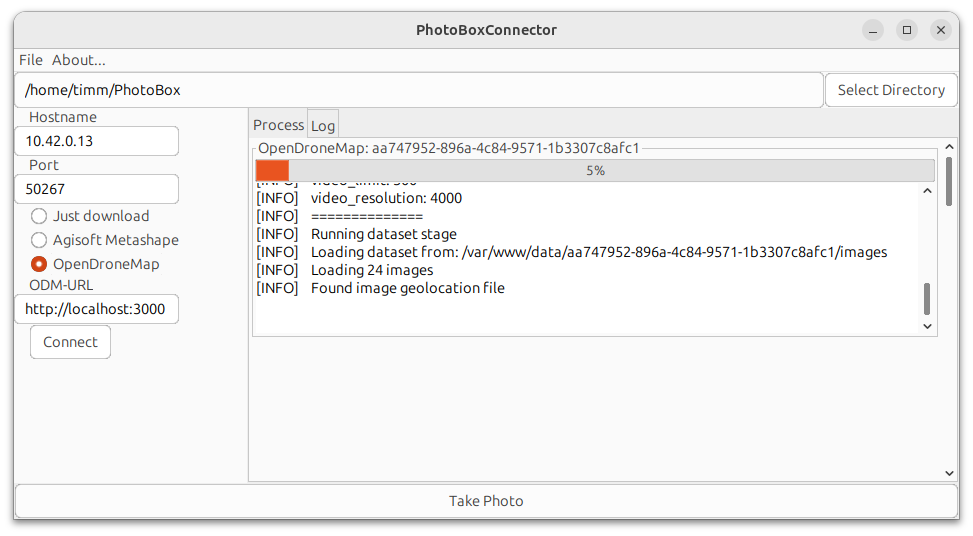
\includegraphics[width=1\textwidth]{./img/connector_screenshot.png}
    \caption{Screenshot der Connector-Software unter Ubuntu 24.04} %Bildunterschrift
    \label{img:screenshot_connector} %ID fürs Bild
\end{figure}

\begin{figure}
    \centering
    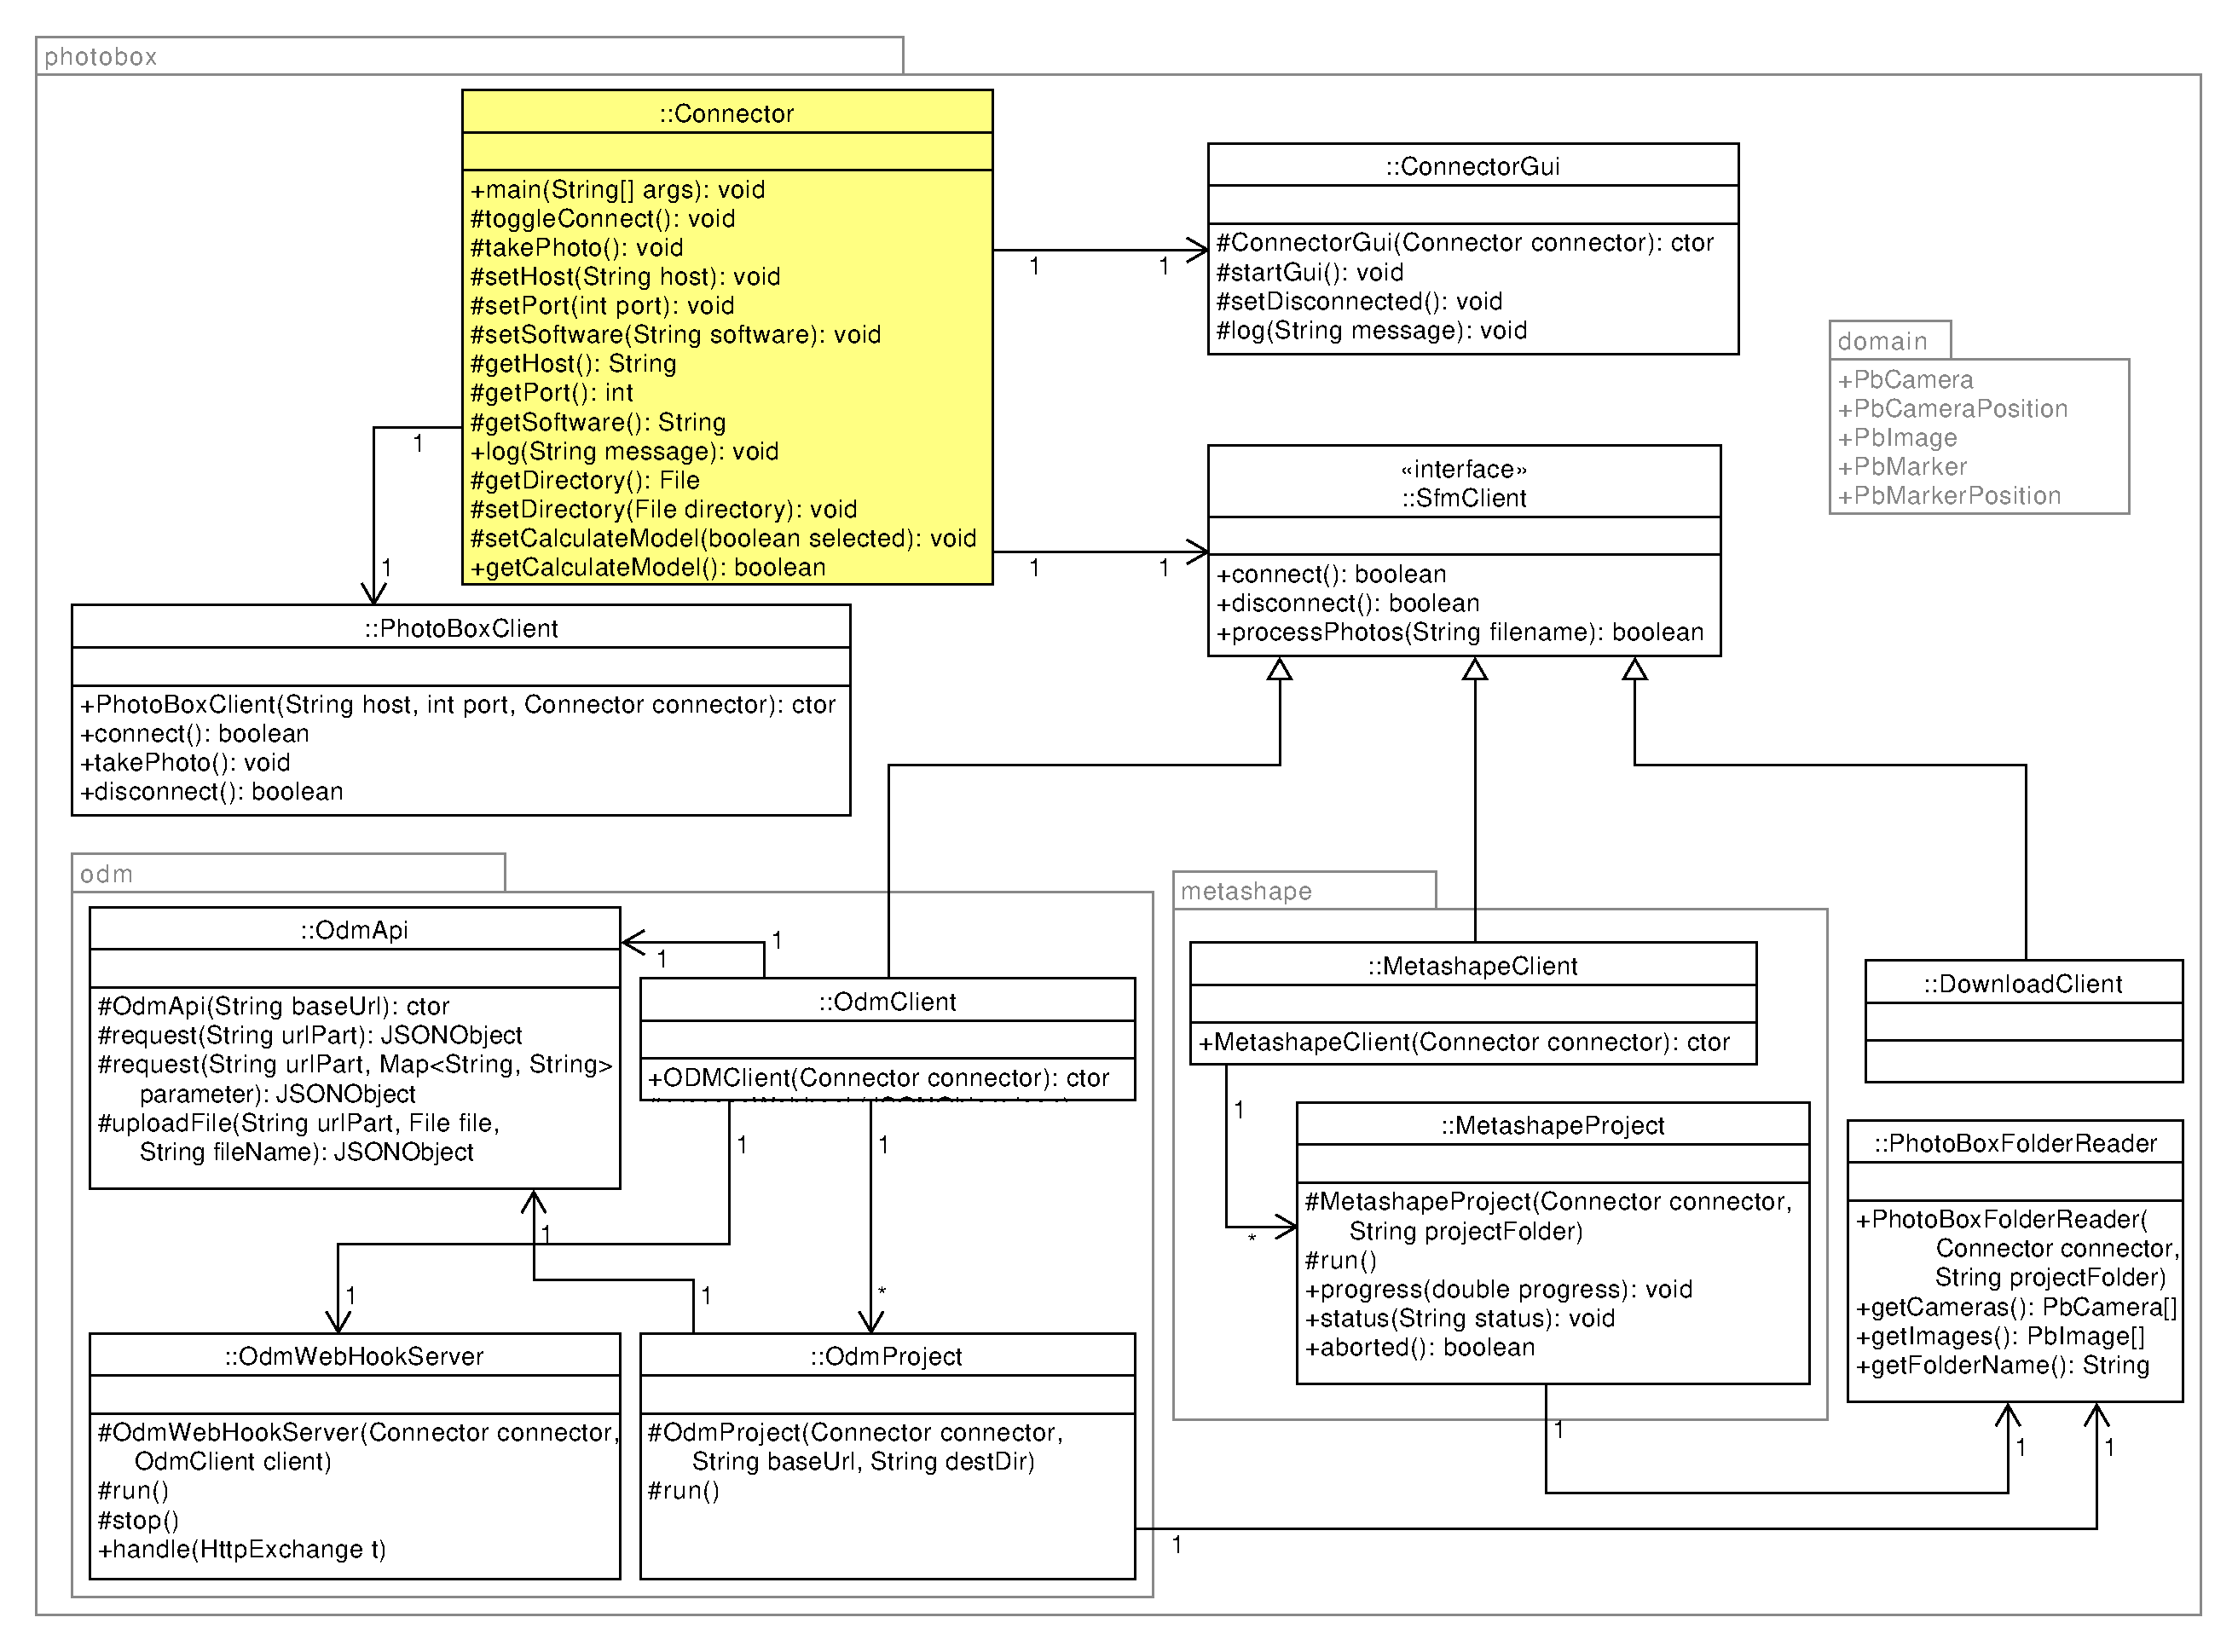
\includegraphics[width=1\textwidth]{./img/uml/uml_connector_classdiagramm.pdf}
    \caption{Connector} %Bildunterschrift
    \label{img:uml_connector} %ID fürs Bild
\end{figure}

\biblio
\end{document}